% GHOST system model with the real intermediate tensors of one request
% (ResNet-20, split after block 3, rho = 10, CIFAR-10 test image 1398), produced by ghost2/fig_tensors.py.
% Drawn at IEEE \textwidth (7.16in) so fonts render at true size.
\documentclass[tikz,border=1pt,10pt]{standalone}
\usepackage[T1]{fontenc}
\usepackage{mathptmx}
\usepackage{courier}
\usepackage{graphicx}
\usetikzlibrary{arrows.meta,calc}
\definecolor{ink}{HTML}{1A1A1A}
\definecolor{dark}{HTML}{263238}
\definecolor{teeC}{HTML}{2E7D32}\definecolor{teeF}{HTML}{EDF6EE}
\definecolor{reeC}{HTML}{C62828}\definecolor{reeF}{HTML}{FCEDED}
\definecolor{clC}{HTML}{1565C0}\definecolor{clF}{HTML}{EAF2FB}
\definecolor{devC}{HTML}{37474F}
\definecolor{acc}{HTML}{E65100}
\definecolor{bar}{HTML}{4A6FA5}
\def\TokHex{e1817c66}
\def\CtHex{d06c51cc}
\def\PredClass{Horse}
\def\ProbList{0.056,0.000,0.013,0.041,0.001,0.066,0.000,0.813,0.008,0.002}
\def\WRows{16}\def\WtRows{20}

\graphicspath{{arch_assets/}}
\tikzset{
  >={Stealth[length=2.1mm,width=1.6mm]},
  font=\footnotesize, every node/.style={text=ink},
  zone/.style={draw=#1,line width=1pt,rounded corners=2.5pt},
  tab/.style={fill=#1,text=white,font=\footnotesize\bfseries,inner xsep=3pt,inner ysep=2pt,rounded corners=1.5pt},
  vtab/.style={fill=#1,text=white,font=\footnotesize\bfseries,rotate=90,inner xsep=4pt,inner ysep=2.5pt},
  ttl/.style={align=center,inner sep=1pt,font=\footnotesize},
  f/.style={->,draw=dark,line width=0.85pt},
  fo/.style={->,draw=dark,line width=0.85pt,dash pattern=on 3pt off 2pt},
  n/.style={circle,draw=dark,line width=0.7pt,fill=white,text=dark,font=\scriptsize\bfseries,inner sep=0pt,minimum size=3.9mm},
  lab/.style={font=\scriptsize,inner sep=1pt},
}
\newcommand{\fstack}[3]{%
  \foreach \k in {3,2,1,0}{%
    \node[inner sep=0pt,anchor=south west,draw=ink,line width=0.35pt]
      at ({#1-0.695+\k*0.13},{#2-0.695+\k*0.13}) {\includegraphics[width=1cm]{#3\k}};}}
\newcommand{\tile}[4]{\node[inner sep=0pt,draw=ink,line width=0.4pt] at (#1,#2) {\includegraphics[width=#4]{#3}};}
\newcommand{\padlock}[2]{%
  \begin{scope}[shift={(#1,#2)}]
   \draw[dark,line width=1.3pt] (-0.11,0.1) -- (-0.11,0.2) arc (180:0:0.11) -- (0.11,0.1);
   \fill[dark,rounded corners=1pt] (-0.19,-0.17) rectangle (0.19,0.12);
   \fill[white] (0,-0.02) circle (0.045);
  \end{scope}}
\newcommand{\cuboid}[5]{% x, y(centre), width, height, colour
  \fill[#5,draw=dark,line width=0.5pt] (#1,#2-#4/2) rectangle ++(#3,#4);
  \fill[#5!70!black,draw=dark,line width=0.5pt] (#1,#2+#4/2) -- ++(0.12,0.12) -- ++(#3,0) -- ++(-0.12,-0.12) -- cycle;
  \fill[#5!85!black,draw=dark,line width=0.5pt] (#1+#3,#2-#4/2) -- ++(0.12,0.12) -- ++(0,#4) -- ++(-0.12,-0.12) -- cycle;}
\begin{document}
\begin{tikzpicture}
% =============================================================== zones
\draw[zone=devC] (0,0.3) rectangle (2.3,6.75);
\node[tab=devC] at (1.15,6.75) {Client};
\draw[zone=devC] (2.55,0.3) rectangle (15.2,6.75);
\node[tab=devC] at (8.9,6.75) {Edge Device};
\draw[zone=teeC,fill=teeF] (2.75,3.55) rectangle (14.85,6.5);
\fill[teeC] (2.75,3.55) rectangle (3.2,6.5);
\node[vtab=teeC] at (2.975,5.025) {TEE (Trusted)};
\draw[zone=reeC,fill=reeF,dash pattern=on 4pt off 2pt] (2.75,0.45) rectangle (14.85,3.35);
\fill[reeC] (2.75,0.45) rectangle (3.2,3.35);
\node[vtab=reeC] at (2.975,1.9) {REE (Adversary)};
\draw[zone=clC,fill=clF] (15.45,0.3) rectangle (18.3,6.75);
\node[tab=clC] at (16.875,6.75) {Model Owner Cloud};
\draw[teeC,line width=1pt,rounded corners=2.5pt] (2.75,3.55) rectangle (14.85,6.5);
\draw[reeC,line width=1pt,rounded corners=2.5pt,dash pattern=on 4pt off 2pt] (2.75,0.45) rectangle (14.85,3.35);

% =============================================================== client
\node[ttl,anchor=north] at (1.15,6.45) {Input and Token};
\tile{1.15}{5.05}{input}{1.25cm}
\node[draw=dark,fill=white,rounded corners=2pt,line width=0.6pt,font=\scriptsize\ttfamily\bfseries,inner sep=2pt] (tok) at (1.15,4.0) {\TokHex};
\draw[dark,line width=0.6pt] (1.15,4.42) -- (tok.north);
\node[ttl,anchor=south] at (1.15,2.85) {Prediction};
\foreach \c [count=\i from 0] in {plane,car,bird,cat,deer,dog,frog,horse,ship,truck}{%
  \pgfmathsetmacro{\p}{{\ProbList}[\i]}
  \pgfmathsetmacro{\yy}{2.67-\i*0.232}
  \node[lab,anchor=east,font=\scriptsize] at (0.8,\yy) {\c};
  \ifnum\i=7
    \fill[acc] (0.85,\yy-0.085) rectangle ++({1.0*\p},0.17);
    \node[lab,anchor=west,font=\scriptsize\bfseries] at ({0.85+1.0*\p},\yy) {\pgfmathprintnumber[fixed,precision=2]{\p}};
  \else
    \fill[bar] (0.85,\yy-0.085) rectangle ++({max(1.0*\p,0.015)},0.17);
  \fi}
\draw[dark,line width=0.6pt] (0.85,2.8) -- (0.85,0.45);

% =============================================================== TEE
\node[ttl,anchor=north] at (4.25,6.45) {Token and\\ Budget Check};
\begin{scope}[shift={(4.25,5.15)}]
  \fill[teeC] (0,0.5) .. controls (0.23,0.41) .. (0.38,0.41) -- (0.38,0.05) .. controls (0.38,-0.27) .. (0,-0.45)
              .. controls (-0.38,-0.27) .. (-0.38,0.05) -- (-0.38,0.41) .. controls (-0.23,0.41) .. cycle;
  \draw[white,line width=1.6pt,line cap=round,line join=round] (-0.18,0.0) -- (-0.04,-0.15) -- (0.2,0.18);
  \foreach \j in {0,...,7}{\ifnum\j<3 \fill[teeC] \else \draw[teeC,line width=0.5pt,fill=white] \fi
     ({-0.62+\j*0.16},-0.78) rectangle ++(0.12,0.19);}
\end{scope}
\node[ttl,anchor=north] at (6.3,6.45) {First\\ Convolution};
\fstack{6.3}{4.95}{a}
\node[ttl,anchor=north] at (8.45,6.45) {Mixing and\\ One-Time Masking};
\fstack{8.45}{4.95}{R}
\node[ttl,anchor=north] at (11.25,6.45) {Unmasking\\ and Unmixing};
\fstack{11.25}{4.95}{y}
\node[ttl,anchor=north] at (13.6,6.45) {Feature\\ Encryption};
\tile{13.6}{5.0}{ct}{0.95cm}
\padlock{13.95}{5.38}
\node[inner sep=1.2pt,draw=teeC,line width=0.9pt,rounded corners=1.5pt,fill=white] (keys) at (13.6,3.98)
  {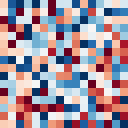
\includegraphics[width=0.48cm]{B}\hspace{2pt}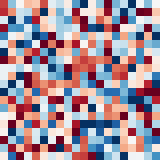
\includegraphics[width=0.48cm]{A}};
\node[ttl,anchor=east] at (keys.west) {Key Store};

% =============================================================== REE
\tile{6.75}{2.2}{Wt}{1.1cm}
\node[ttl,anchor=east] at (6.15,2.2) {Obfuscated\\ Weights};
\fstack{8.45}{2.25}{xt}
\node[ttl,anchor=north] at (8.45,1.5) {Masked Activation};
\begin{scope}[shift={(9.85,2.1)}]
  \foreach \j in {-0.2,-0.07,0.07,0.2}{
    \draw[dark,line width=0.6pt] (\j,0.3) -- (\j,0.4); \draw[dark,line width=0.6pt] (\j,-0.3) -- (\j,-0.4);
    \draw[dark,line width=0.6pt] (0.3,\j) -- (0.4,\j); \draw[dark,line width=0.6pt] (-0.3,\j) -- (-0.4,\j);}
  \fill[dark,rounded corners=1.2pt] (-0.3,-0.3) rectangle (0.3,0.3);
  \fill[acc] (-0.14,-0.14) rectangle (0.14,0.14);
\end{scope}
\node[ttl,anchor=south] at (9.85,2.52) {Accelerator\\ Convolution};
\fstack{11.25}{2.25}{yt}
\node[ttl,anchor=north] at (11.25,1.5) {Masked Output};
% adversary side information
\node[ttl,font=\footnotesize\bfseries,text=reeC] at (13.55,2.93) {Adversary Knowledge};
\tile{12.95}{2.12}{aux}{0.95cm}
\node[ttl,anchor=north] at (12.95,1.57) {Auxiliary\\ Data};
\tile{14.15}{2.12}{Wref}{0.95cm}
\node[ttl,anchor=north] at (14.15,1.57) {Reference\\ Model};

% =============================================================== cloud
\node[ttl,anchor=north] at (16.875,6.45) {Suffix Network};
\fstack{16.3}{4.95}{f}
\cuboid{17.13}{4.95}{0.2}{0.85}{clC}
\cuboid{17.48}{4.95}{0.18}{0.62}{clC}
\cuboid{17.8}{4.95}{0.15}{0.4}{clC}
\foreach \t/\yy/\s in {Probability Vector/3.78/1,Top-1 Confidence/3.43/0,Label Only/3.08/0}{
  \ifnum\s=1 \node[fill=clC,text=white,rounded corners=1.9mm,font=\scriptsize\bfseries,minimum width=2.45cm,inner ysep=1.6pt] at (16.875,\yy) {\t};
  \else \node[draw=clC,fill=white,rounded corners=1.9mm,font=\scriptsize,line width=0.6pt,minimum width=2.45cm,inner ysep=1.6pt] at (16.875,\yy) {\t}; \fi}
\node[ttl,anchor=north] at (16.875,2.88) {Output Release Policy};
\tile{16.875}{1.12}{W}{1.0cm}
\node[ttl,anchor=south] at (16.875,1.65) {Attestation and\\ Provisioning};

% =============================================================== legend
\draw[f] (3.5,1.3) -- ++(0.55,0) node[right,lab]{Online inference};
\draw[fo] (3.5,0.92) -- ++(0.55,0) node[right,lab]{One-time setup};

% =============================================================== one-time setup
\draw[fo] (16.375,0.65) -- (6.4,0.65) -- (6.4,1.65);
\draw[fo] (16.375,1.3) -- (15.02,1.3) |- (keys.east);

% =============================================================== online inference
\draw[f] (1.775,5.05) -- node[pos=0.33,n,above=2pt]{1} (3.8,5.05);
\draw[f] (4.7,5.05) -- node[n,above=2pt]{2} (5.6,5.05);
\draw[f] (7.0,5.05) -- (7.75,5.05);
\draw[f] (8.45,4.25) -- node[n,left=2pt]{3} (8.45,2.95);
\draw[f] (9.15,2.1) -- (9.4,2.1);
\draw[f] (10.3,2.1) -- (10.55,2.1);
\draw[f] (7.1,1.65) -- (7.1,0.92) -| (9.85,1.65);
\draw[f] (11.25,2.95) -- node[n,right=2pt]{4} (11.25,4.25);
\draw[f] (10.55,5.05) -- node[n,above=2pt]{5} (9.15,5.05);
\draw[f] (11.95,5.05) -- node[n,above=2pt]{6} (13.12,5.05);
\draw[f] (14.08,5.05) -- node[n,above=2pt]{7} (15.6,5.05);
\draw[f] (16.875,4.25) -- (16.875,3.97);
\draw[f] (18.1,3.78) -- (18.15,3.78) -- (18.15,0.05) -| node[pos=0.25,n,below=1.5pt]{8} (1.15,0.5);
\end{tikzpicture}
\end{document}
